% -*- root: ./report.tex -*-
\chapter{Introduction}

\comment{The history of quantum computing and why QC is important}
	The idea of using coherent quantum states as a means to perform complex calculations first appeared in the beginning of the 80's.
	A handful of papers had already been published on the matter, when, during a keynote speech~\cite{feynman_simulating_1982} at the California Institute of Technology, Nobel laureate Richard Feynman suggested its importance with respect to physics simulations.
	To put his idea in very simple terms, calculating the quantum mechanical state of a system on a conventional computer scales exponentially with respect to the system size.
	By making a computer that is based on quantum states itself, and creating a mapping between those states and the system you want to simulate, this scaling becomes polynomial.
	Beyond their significance in physics simulations, quantum computers could be used in a more pragmatic way, for implementing cryptography, optimization and search algorithms.
	With the potential applications in mind, a lot of resources and effort have been put into building such a quantum computer in the last years.
	Recently, apart from being a largely publicly funded effort, the private sector has also started to recognize the potential of this technology: large companies such as Microsoft~\cite{noauthor_why_nodate}, Google~\cite{noauthor_quantum_nodate} and IBM~\cite{noauthor_ibm_2018} are investing into the development of a quantum computer.
	As of this moment, functional quantum computers have been realized on a very small scale: calculations of meaningful magnitude are still not possible.

\comment{It is still an open question what the implementation for a qubit will be, but majorana's are one of the contenders}
	If we consider the evolution of the regular computer, we see that the technological/physical platform for the bit, the binary unit of information, has been constantly changing.
	For the earliest computers, complex electromechanical systems with gears and cogs fulfilled this role.
	Soon after, binary states were implemented in the form of vacuum tubes, and nowadays it is the transistor which acts as the basic unit of computation.
	Similarly, because quantum computing is still in its infancy, there are still many contenders for what the underlying technology will be: what physical system will form the basis for the quantum bit, the qubit?
	The platforms which are currently explored for the implementation of a qubit include the transmon qubit~\cite{wendin_quantum_2017}, NV-centers~\cite{childress_diamond_2013}, quantum dots~\cite{kloeffel_prospects_2013}, and Majorana bound states~\cite{wendin_quantum_2017}.
	The main problem with most of the quantum computing platforms is that it is very difficult to keep the qubit from decohering.
	To counteract this, apart from trying to reduce the decoherance rate of the qubit, much effort is put into devising quantum error correction codes: devise strategies such that potential errors can be detected and corrected for.
	For topological quantum computers, employing Majorana bound states as qubits, information is encoded in such a way that it is inherently protected against decoherence.
	This \emph{topological} protection of the quantum states makes Majorana bound states (MBSs) a promising candidate as a stable platform for quantum computing.
	However, the implementation of such Majorana bound states has proven elusive, and much research is being done on designing a device that reliably and unequivocally hosts Majoranas.
	In this manuscript, we devise a novel way to improve the reliability of such devices, while remaining compatible with current fabrication techniques.

\section{Majorana bound states as qubits}

	\comment{What are Majorana bound states}
	Majorana particles are particles that always come in pairs: one pair of Majorana's forms a single electronic state.
	Disambiguating electrons and holes into their Majorana counterparts is analogous to splitting a complex number into its real and imaginary part.
	We write the Majorana operators in terms of the creation (annihilation) and annihilation (creation) operators of electrons (holes), respectively $\hat{c}^\dagger$ and $\hat{c}$:

	\begin{align}
		\hat{c} =  \frac{1}{2} \left( \gamma_1 - i\gamma_2 \right) && \hat{c}^\dagger = \frac{1}{2} \left( \gamma_1 + i\gamma_2 \right)
		\label{eq:intro_ferm2maj}
	\end{align}

	Inverting this, we obtain,
	\begin{align}
		\gamma_1 = \hat{c} + \hat{c}^\dagger && \gamma_2 = i \left( \hat{c} - \hat{c}^\dagger \right)
		\label{eq:intro_maj2ferm}
	\end{align}

	Note that the basic excitation is still a fermion (electron/hole); one cannot have just one Majorana, they always come in pairs.
	The idea is to create a system where we have a single pair of Majoranas which is separated in space.

	A system in which this separation can be accomplished was first proposed by Kitaev~\cite{kitaev_unpaired_2001}.
	We consider a one dimensional chain of sites which can host a single fermion, and thus a pair of Majoranas.
	Suppose that the occupation of a site by a fermion comes at the cost of energy $\mu$.
	Also, we consider the situation where there is an interaction energy between neighboring sites: $t$ quantifies the energy cost of one site being occupied while the adjacent is not, and $\Delta$ is the gain in energy if adjacent sites are both occupied or empty.
	This leads to the following Hamiltonian:

	\begin{equation}
		H = -\mu \sum_n \hat{c}_n^\dagger \hat{c}_n
		- t \sum_n \left( \hat{c}_{n+1}^\dagger \hat{c}_n +\text{h.c.} \right) 
		+ \Delta \sum_n \left( \hat{c}_n \hat{c}_{n+1} +\text{h.c.} \right) 
	\end{equation}

	Considering equation \eqref{eq:intro_ferm2maj} we can also write the Hamiltonian above using Majorana operators.
	In this way, we get a Hamiltonian describing pairing energies between Majoranas on adjacent sites.
	We discern two extremes: In figure \ref{fig:trivial_majoranas}, the situation where the pairing energy is minimal for Majorana pairs on the same site:
	\begin{figure}[htb!]
	\centering
	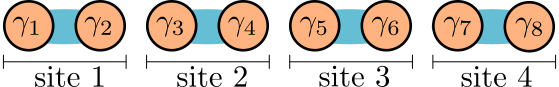
\includegraphics[width=0.95\columnwidth]{images/majorana_trivial_pairing}
	\caption{Trivial Majorana pairing in a Kitaev chain}
	\label{fig:trivial_majoranas}
	\end{figure}

	The other is when the energy is minimal for pairing between of Majoranas from adjacent sites:
	\begin{figure}[htb!]
	\centering
	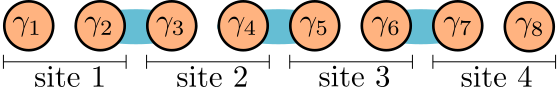
\includegraphics[width=0.95\columnwidth]{images/majorana_topological_pairing}
	\caption{Topological Majorana pairing in a Kitaev chain}
	\label{fig:topological_majoranas}
	\end{figure}
		
	As is apparent from the above image, this would leave two unpaired Majoranas at the ends of the chain.
	This is the state we are interested in: the Majorana state, where two Majoranas are separated in space.
	This physical separation has the effect of not allowing simple local perturbations to disturb the system, thus inherently protecting the system against decoherence.

\section{Ways to make Majorana's: nanowires \& sns system}
	A realistic experimental implementation of Kitaev's model did not emerge until the similar works of Lutchyn et. al~\cite{lutchyn_majorana_2010} and Oreg et. al~\cite{ oreg_helical_2010}, where they proposed an experiment composed of a semiconducting nanowire deposited onto a superconductor.
	They predicted that, if the semiconductor has strong spin-orbit coupling, a magnetic field applied along the wire axis, as well as a carefully tuned chemical potential, Majoranas would appear at the ends of the nanowire.
	The experiment proved to be sufficiently practical to perform in the lab and the first signatures of Majorana bound states were found using the setup by Mourik et. al~\cite{mourik_signatures_2012}.

	For the same reasons Majoranas are inherently protected against decoherence, it is notoriously difficult to prove their existence.
	Perhaps the most direct way to detect their presence is through the observation of a so-called zero bias peak.
	When performing a tunneling conductance experiment, measuring the conductance through the nanowire, the zero-energy (with respect to the Fermi energy) Majorana state provides a resonant tunneling state when no bias is applied, appearing as a peak in conductance.
	There are however also other physical phenomena which can be responsible for such a conductance peak, and thus it is not unique to the Majorana state.

\section{Majoranas in a Josephson junction}
	\comment{Why are SNS junctions potentially better?}
	A more convincing case could be made if one could control the system in such a way that the presence of Majoranas can be turned on or off.
	This feature is realized in a relatively recent proposal by Pientka et. al~\cite{pientka_topological_2017}, where, instead of a nanowire, a two-dimensional strip of semiconductor is used.
	On each side of the strip a superconductor is placed, forming a Josephson junction.
	Using the Josephson junction, one can use the supercurrent which flows between the two superconductors to control whether the system is in a topological phase (meaning it contains Majoranas), or not.
	The system has addition advantages, namely the system allows for Majorana's to be created at lower magnetic fields, the system is more compatible with convential semiconductor technology, and the Josephson junction allows for new ways to detect the topological phase of the system.

	% \comment{Current experimental progress}
	% Two papers that claimed they have observed signs of topological behavior.
	% Soft gap, questionable results.

	\comment{The challenges encountered}
	One of the biggest challenges in creating stable Majoranas is the appearance of a soft gap; where the gap in the density of states is greatly reduced for states with the momentum directed along the length of the strip.
	From a semiclassical perspective, these momenta correspond to long paths through the semiconductor without interruption by the superconductor.
	Additionally, these long trajectories have long flight times $\tau_f$ and equivalenly small Thouless energies $E_{\textrm{Th}}=\hbar / \tau_f$, resulting in a small gap. 
	Currently, proposed workarounds are low density or disorder~\cite{haim_double-edge_2018}, but both have drawbacks.


	We propose that the introduction of a zigzag-shaped modulation of the junction region leads to an increased topological gap, as well as a reduction of the Majorana coherence length.
	Furthermore, we hypothesize that the gap improvement is the result of the elimination of long trajectories